\documentclass[a4paper]{article}
\usepackage[T1]{fontenc}
\usepackage[a4paper,margin=3cm]{geometry}
\usepackage{anyfontsize}
\usepackage{graphicx}
\usepackage{subcaption}
\usepackage[ngerman]{babel}
\usepackage[backend=biber,style=numeric,defernumbers=true, sorting=none]{biblatex} 
\usepackage{amsmath}
%\usepackage{svg}
\usepackage{hyperref}
\usepackage{caption}
\usepackage{csquotes}
\usepackage{lmodern}

\setcounter{biburllcpenalty}{7000}
\usepackage{listings}
\usepackage{xcolor}

% Definieren der Farben für den Code
\definecolor{codegreen}{rgb}{0,0.6,0}
\definecolor{codegray}{rgb}{0.5,0.5,0.5}
\definecolor{codepurple}{rgb}{0.58,0,0.82}
\definecolor{backcolour}{rgb}{0.95,0.95,0.92}

% Stil für Python-Code festlegen
\lstdefinestyle{mystyle}{
    backgroundcolor=\color{backcolour},   
    commentstyle=\color{codegreen},
    keywordstyle=\color{magenta},
    numberstyle=\tiny\color{codegray},
    stringstyle=\color{codepurple},
    basicstyle=\ttfamily\footnotesize,
    breakatwhitespace=false,         
    breaklines=true,                 
    captionpos=b,                    
    keepspaces=true,                 
    numbers=left,                    
    numbersep=5pt,                  
    showspaces=false,                
    showstringspaces=false,
    showtabs=false,                  
    tabsize=2,
    language=Python
}
\lstset{style=mystyle}


% Quellen
\addbibresource{Quellen.bib}

\title{ Lineare Anamorphose }
\author{Daniel Stumpp}
\date{ \today } %TODO akutell halten

\begin{document}

%Titelseite
\begin{titlepage}
    \centering

    \noindent
    \hspace*{\fill}
    \begin{minipage}[t]{0.4\textwidth}
        \flushright
        
\includegraphics[width=\textwidth]{img/logo_uulm_sw.png}
    \end{minipage}

    \vspace{1cm}
    
    {\huge Die perspektivische Anamorphose nach Niceron und algorithmische Umsetzung in Manim \par}
    \vspace{1cm}
    
    {\large Daniel Stumpp \par}
    \vspace{1cm}
    
    {\large \today \par}
    \vspace{2cm}

\end{titlepage}

\newpage
\tableofcontents % <--- Hier wird das Verzeichnis erstellt
\newpage

%Einleitung/historische Einordnung
\section{Historische Einordnung}

Obwohl ausreichend Werke - vor allem Gemälde - existieren, um Italien im \textit{Quattrocento} als Geburtsort der Perspektive zu bestimmen, betont Andersen eine entscheidende Lücke: Es gebe keinerlei Dokumente, die die einzelnen Entwicklungsschritte früherer Generationen belegen. Diese Kluft führte in der Forschung zu zahlreichen Spekulationen. \footnote{Vgl.: \cite[S. 2]{Andersen2007}}
Die Entstehung der Perspektive wird als ein Meilenstein der Menschheitsgeschichte betrachtet. Ich werde mich darauf konzentrieren, einzelne Aspekte zu beleuchten, die zur Geburt der Perspektive beigetragen haben könnten. Sobald wir die historische Perspektive als das notwendige Fundament etabliert haben, lässt sich darauf das mathematisch-historische Gebäude errichten, welches uns schließlich erlaubt, die "`Magie"' dieser Entwicklung -- die \textit{perspektivische Anamorphose} -- fachgerecht zu analysieren und zu begreifen.
Den Ursprung der mathematischen Theorie der Perspektive markiert der italienische Universalgelehrte Leon Battista Alberti, der in seinem Werk \textit{De pictura} um 1435 erstmals ein Modell zum perspektivischen Zeichnen festhielt.\footnote{Vgl.: \cite[S. 1]{Andersen2007}}

Ausgehend von Albertis Konzepten systematisierte der italienische Mathematiker Piero della Francesca im späten 15. Jahrhundert mit seinem Traktat \textit{De prospectiva pingendi} die Grundriss-Aufriss-Methode. \footnote{Vgl.: \cite[S. 14]{Andersen2007}} Mithilfe dieses Verfahrens konstruierte Piero explizit die erste perspektivische Anamorphose - eine gezielte zeichnerische Verzerrung, die erst aus einem speziellen Blickwinkel ihre korrekte Form preisgibt. \footnote{Vgl.: \cite[S. 71-73]{Andersen2007}}

Die neue Darstellungsform wanderte im folgenden Jahrhundert über die Alpen in nördlichere Gebiete ein, darunter auch nach Frankreich und Deutschland.

Angetrieben von der Neugierde an Synthesen aus Geometrie und Optik, eröffnete das  Lehrbuch  \textit{La perspective curieuse, ou magie artificiele des effets merveilleux} (1638) des Minim-Priesters Jean François Niceron (1613–1646) die anamorphotische Kunst auch für Laien: \footnote{Vgl.: \cite[S. 452]{Andersen2007}}

\enquote{TOVTES les parties des Mathematiques ont de rares inuentions, \& des subtilitez qui les ont fait estimer \& cultiuer par les plus beaux esprits de l'antiquité, \& qui les font encore aujourdhuy rechercher par les plus curieux de nostre siecle.} \footnote{\cite[S. 1]{Niceron1663}. dt. Übersetzung: "`Alle Teilbereiche der Mathematik bergen seltene Erfindungen und Feinheiten, derentwegen sie von den feinsten Geistern der Antike geschätzt und gepflegt wurden, und die bewirken, dass sie auch heute noch von den Neugierigsten unseres Jahrhunderts erforscht werden. "'}
 \newpage

%Mathematische Ideen (TODO Titel)
\section{Mathematische Ideen}

Andersen betont, dass Maler über die reine Beobachtung hinausgingen und stattdessen angespornt waren, jene mathematische Regeln zu formulieren, nach denen sich der Raum organisierte. \footnote{Vgl.: \cite[S. 3]{Andersen2007}}
Um 1435 definierte Leon Battista Alberti in seinem Werk \textit{De pictura} das perspektivische Bild erstmals mathematisch als den direkten Schnitt der Sehpyramide mit der Bildebene. Der Eindruck des Gemäldes sollte dieselbe Tiefe suggerieren, als betrachte man eine Szene durch ein geöffnetes Fenster. \footnote{Vgl.: \cite[S. 1]{Andersen2007}} Während Alberti die \textit{Konvergenzregel} - das ist jene Regel, nach der sich alle Tiefenlinien (Orthogonalen) in einem gemeinsamen Fluchtpunkt treffen, dem \textit{Hauptfluchtpunkt} - stillschweigend voraussetzte, lieferte Guidobaldo del Monte im Jahr 1600 den mathematischen Beweis. Rückblickend lässt sich sagen, dass diese Entwicklung die korrekte räumliche Darstellung geometrischer Körper, wie Polyeder oder architektonischer Elemente, erst ermöglichte. \footnote{Vgl.: \cite[S. 4-9]{Andersen2007}}

Sei $\pi$ die Bildebene und $O$ ein Augpunkt. Die Abbildungsvorschrift ist, dass jeder Punkt $A$ hinter der Bildebene $\pi$ auf einen Punkt $A_i$ auf der Bildebene abgebildet wird, und zwar als Schnittpunkt der Geraden $OA$ mit $\pi$. \footnote{Vgl.: \cite[S. 1]{Andersen2007}}

Um ein dreidimensionales Objekt zu beschreiben, ist zu beachten, dass Albertis Konstruktionsmethode nur teilweise auf einer Grundriss- und Aufriss-Methode basierte und die älteste bekannte Beschreibung dieses Verfahrens von Piero della Francesca stammt. \footnote{Vgl.: \cite[S. 14]{Andersen2007}}

Sei $O$ der Augpunkt des Betrachters und $B$ ein beliebiger Punkt des Objekts im Raum. Sei außerdem $\pi$ die vertikale Bildebene (Leinwand) und $b$ der Durchstoßpunkt des Sehstrahls $OB$ durch die Bildebene $\pi$.

Um diesen 3D-Schnittpunkt $b$ auf einem flachen Blatt Papier identifizieren zu können, projizierte Piero die gesamte Konfiguration auf zwei orthogonale Hilfsebenen: Sei $\gamma$ (Grundriss) die horizontale Bodenebene und $\epsilon$ (Aufriss) die vertikale Ebene, die senkrecht auf dem Grundriss $\gamma$ und senkrecht auf der Bildebene $\pi$ steht. 

Die resultierenden Schnittlinien $GR$, $GT$ und $GH$ der Ebenen bilden das Koordinatensystem.

Anstatt den Schnittpunkt $b$ im dreidimensionalen Raum zu berechnen, projizierte Piero den Punkt $O$, den Punkt $B$ und den gesuchten Bildpunkt $b$ jeweils orthogonal auf den Grundriss und den Aufriss. 

Im Grundriss werden der Augpunkt und der Objektpunkt auf $O_p$ und $B_p$ abgebildet, der Sehstrahl $OB$ zu $O_pB_p$ und $b$ zu $b_p$. Da die Leinwand $\pi$ von oben nur als die Gerade $GR$ erscheint, ist die Projektion des Bildpunktes $b_p$ exakt der Schnittpunkt zwischen den Geraden $O_pB_p$ und $GR$. 

Im Aufriss werden der Augpunkt und der Objektpunkt als $O_e$ und $B_e$ abgebildet. Die Bildebene $\pi$ erscheint in der vertikalen Ansicht nur als die Linie $GT$, womit die Projektion des Bildpunktes $b_e$ exakt der Schnittpunkt zwischen $O_eB_e$ und $GT$ ist.

Im nächsten Schritt drehte er die vertikale Aufrissebene $\epsilon$ um die Achse $GH$ nach unten, bis sie flach in derselben Ebene wie der Grundriss $\gamma$ lag. Sobald $B_p$, $B_e$, $O_p$ und $O_e$ auf dem Papier bekannt sind, können daraus die Punkte $b_p$ und $b_e$ durch einfaches Ziehen von Linien konstruiert werden. 

Während die horizontale Position des Leinwandpunktes $b$ sich aus der Distanz auf der Gerade $GR$ ergibt, berechnet sich die vertikale Höhe des Punktes aus der Distanz $Gb_e$ auf der vertikalen Linie $GT$. Indem man eine Senkrechte durch $b_p$ (nach oben) und eine Senkrechte durch $b_e$ (zur Seite) zieht, erhält man am Schnittpunkt dieser beiden Linien den finalen Punkt $b$. \footnote{Vgl.: \cite[S. 60-63]{Andersen2007}}

Piero verstand die Mathematik der Zentralprojektion so tiefgreifend, dass er die geometrischen Parameter bewusst veränderte: Stellen wir uns vor, die Leinwand liegt flach auf einem Tisch. Erinnern wir uns an Albertis Perspektiv-Modell, so wird deutlich, dass ausgehend von einem Augpunkt O eine Sehpyramide mit der Bildebene geschnitten wird. Indem wir den Augpunkt extrem flach nahe zur Tischkante führen, unterliegt die resultierende Bildebene einer extremen Verzerrung. Dies hat zur Folge, dass seine Zeichnungen nur dann unverzerrt erscheinen, wenn sie exakt aus dem von Piero kalkulierten Augpunkt betrachtet werden - die erste perspektivische Anamorphose ist entstanden. \footnote{Vgl.: \cite[S. 74-75]{Andersen2007}}

Um 1623 veröffentlichte der Ingenieur und Rechenmeister Andreas Albrecht (1586--1628) mit seinem Werk \textit{Zwey Bücher} das erste deutschsprachige Werk, welches die Konstruktion von perspektivischen Anamorphosen -- von ihm \textit{Ongestalt} genannt -- behandelte. Im Gegensatz zu Pieros Grundriss-Aufriss-Methode verwendete er einen arithmetischen Ansatz, für den er aufwendig ein umfangreiches Tabellenwerk ausarbeitete.\footnote{Vgl.: \cite[S. 605-606]{Andersen2007}}

Sei $\pi$ eine vertikale Bildebene. Wir definieren den Augpunkt $O$ und nennen seine orthogonale Projektion auf die Grundebene $O'$. Die Höhe des Augpunktes über der Grundebene sei $h$ (Strecke $OO'$). Der orthogonale Abstand des Augpunktes zur Bildebene $\pi$ sei $d$. Sei nun $C$ ein beliebiger, zu projizierender Raumpunkt und $A$ seine senkrechte Projektion auf die Grundebene. Die Position des Punktes $C$ wird wie folgt definiert: $a$ als der räumliche Tiefenabstand von $A$ zur Bildebene $\pi$, $b$ als der laterale Abstand von $A$ zur zentralen Vertikalebene (die durch $O$ und $O'$ verläuft) und $c$ als die Höhe des Punktes $C$ über der Grundebene (Strecke $AC$). 

Für die Bestimmung der projizierten Koordinaten ($x$, $y$ und $z$) in der Bildebene $\pi$ nutzte Albrecht die geometrischen Gesetzmäßigkeiten des Strahlensatzes, indem er die Sichtstrahlen vom Augpunkt $O$ zu den Objektpunkten ($A$ und $C$) im Raum betrachtete. Durch den Schnitt dieser Sichtstrahlen mit der Bildebene entstehen ähnliche Dreiecke. Folglich entspricht das Verhältnis der projizierten Strecken auf der Bildebene zu den Originalstrecken im Raum dem Verhältnis der Sehdistanz $d$ zur Gesamttiefe ($a+d$).

Durch algebraische Äquivalenzumformungen leitete Albrecht daraus die finalen anamorphotischen Abbildungsgleichungen ab, um seine Tabellen zu berechnen: 
$$x = \frac{d \cdot b}{a+d}, \quad y = \frac{a \cdot h}{a+d} \quad \text{und} \quad z = \frac{d \cdot c}{a+d}$$

Während Albrechts Tabellenwerk für den gewöhnlichen Maler kaum zu dechiffrieren war, beabsichtigte Jean-François Niceron mit seiner Arbeit eine detaillierte Anleitung zur Konstruktion perspektivischer Anamorphosen, die selbst für Laien zugänglich sein sollte. \footnote{Vgl.: \cite[S. 452]{Andersen2007}} 

Das grundlegende Prinzip für die Konstruktion eines anamorphotischen Rasters bildet Nicerons Konstruktion aus \textit{La perspective curieuse}. 
Sei $\epsilon$ eine vertikale Ebene im Raum mit einem Rasterfeld und einer Diagonale $LN$. Sei außerdem $O$ ein fest definiertes Projektionszentrum im dreidimensionalen Raum (Augpunkt des Betrachters). 

Sei der Hauptpunkt $P$ definiert als die orthogonale Projektion des Augpunktes $O$ auf die Projektionsebene $\pi$. Der Distanzpunkt $D$ liegt ebenfalls auf $\pi$, wobei sein Abstand zu $P$ der Sehdistanz entspricht, sodass für die Streckenlängen gilt: $|DP| = |OP|$. Dies impliziert, dass $P$ der Hauptfluchtpunkt ist. Da die Tiefenlinien (Horizontalen) des unverzerrten Rasters in $\epsilon$ orthogonal zur Bildebene $\pi$ stehen, werden sie auf Geraden projiziert, die sich im Hauptfluchtpunkt $P$ schneiden.

Die Querlinien (Vertikalen) des Rasters in $\epsilon$ verlaufen parallel zur Bildebene $\pi$. Ihre anamorphotische Abbildung wird durch die Diagonale $LN$ determiniert. Diese Diagonale verläuft im Originalraster in einem $45^\circ$-Winkel zu den Tiefenlinien. Ihr Startpunkt $L$ liegt auf der Schnittgeraden von $\epsilon$ und $\pi$. Da der Distanzpunkt $D$ die korrekte Sehdistanz repräsentiert, fungiert er als Fluchtpunkt für alle $45^\circ$-Diagonalen. Folglich ist die Projektion der Diagonale auf $\pi$ exakt die Strecke $LD$. Die gesuchten Positionen der vertikalen Querlinien im verzerrten Raster ergeben sich aus den Schnittpunkten der projizierten Diagonale $LD$ mit den im Hauptfluchtpunkt $P$ zusammenlaufenden Tiefenlinien.

Sein Ordensbruder Emmanuel Maignan (1601-1676) nutzte dieses Wissen, um monumentale anamorphotische Wandbilder zu erschaffen. Ein herausragendes Beispiel hierfür ist das Fresko im Kloster \textit{Trinità dei Monti} in Rom: Betrachtet man es aus dem exakt definierten Augpunkt, offenbart sich das Porträt des Ordensgründers Franz von Paola. Aus anderen Blickwinkeln betrachtet, zeigt die Wandbemalung hingegen eine Darstellung seiner gefährlichen Überquerung der \textit{Straße von Messina}. \footnote{Vgl.: \cite[S. 455-457]{Andersen2007}}

\newpage

\section{Kultureller und technischer Kontext}

Auf der Suche nach einer unmittelbaren räumlichen Realität experimentierte der italienische Künstler Duccio di Buoninsegna (ca. 1255–1319) mit der perspektivischen Darstellung. In seinem Werk \textit{Das Letzte Abendmahl} (ca. 1310) zeichnete er erste Linienpaare mit einem eigenen Fluchtpunkt, während in dem späteren Werk \textit{Ankündigung des Todes der Jungfrau} (1310) schließlich alle Deckenlinien in einem Hauptfluchtpunkt zusammenlaufen. \footnote{Vgl.: \cite[S. 4-9]{Andersen2007}}

Als Begründer der eigentlichen Perspektive im zweiten Jahrzehnt des \textit{quattrocento} gilt jedoch Filippo Brunelleschi (1377–1446). Laut frühen Biografien demonstrierte er seine Erfindung auf zwei Holztafeln, welche die Kirche \textit{San Giovanni} und den \textit{Palazzo dei Signori} in Florenz zeigten. Für die erste Holztafel nutzte Brunelleschi einen Spiegel, über den der Beobachter auf das Spiegelbild des Baptisteriums blickte, was den Anspruch untermauerte, eine exakte Momentaufnahme der Wirklichkeit zu reproduzieren. Trotz dieser historischen Bedeutung bleibt bis heute unklar, woher er die Inspiration für seinen Aufbau fand oder welche mathematische Konstruktionsmethode er für die Holztafeln anwandte, da die Originale verloren gingen. Ausgehend von einer Gruppe Florentiner Künstler verbreitete sich Brunelleschis Innovation jedoch über ganz Italien, sodass die Zentralperspektive bis zum Ende des 16. Jahrhunderts zu einem allgemeingültigen Paradigma für die folgenden 300 Jahre avancierte. \footnote{Vgl.: \cite[S. 11-14]{Andersen2007}}

Die perspektivische Anamorphose als gezielte zeichnerische Verzerrung entsprach in der Folge exakt der Vorliebe des Manierismus für das Mysteriöse. \footnote{Vgl.: \cite[S. 71-75]{Andersen2007}} In dieser Epoche erlangten Künstler wie Giuseppe Arcimboldo (1527-1593) durch Werke wie \textit{Vertumnus} (1590) Berühmtheit, indem sie Porträts rein aus Objekten wie Früchten oder Blumen komponierten. \footnote{Vgl.: \cite{Kemp1990}} Während solche manieristischen Werke oft auf einer spielerischen Verzerrung durch einfache Rastermethoden beruhten, unterschied sich dies deutlich von der mathematischen Präzision der direkten Konstruktion nach Piero della Francesca. \footnote{Vgl.: \cite[S. 74-75]{Andersen2007}}

Ihren Höhepunkt fand diese Entwicklung schließlich in den Arbeiten des Minim-Priesters Jean-François Niceron sowie des Jesuiten Athanasius Kircher und dessen Schüler Gaspar Schott. Sie nutzten diese optischen Wunderwerke im Kontext der „natürlichen Magie“ und der Illusionskunst primär für didaktische und religiöse Zwecke, um Wissen auf faszinierende Weise zu vermitteln. \footnote{Vgl.: \cite[S. 609-611]{Andersen2007}}

\newpage

\section{Visualisierung mit Manim}

Ziel dieses Kapitels war es, das anamorphotische Distanzpunktverfahren nach Niceron algorithmisch in Manim zu implementieren. Dafür wurde ein objektorientierter Ansatz in Python gewählt, mit dem hochauflösende Phasenbilder für jede einzelne Konstruktionsphase generiert wurden.

In den ersten beiden Konstruktionsschritten (vgl. Abb. 1a und 1b) etabliert das Skript das räumliche Fundament und die Tiefenlinien. Hierzu werden der Hauptfluchtpunkt $P(0,3)$ und der Distanzpunkt $D(4,3)$ in einem diskreten Koordinatensystem definiert. Anschließend generiert eine iterative Schleife die orthogonalen Tiefenlinien, welche alle im Hauptfluchtpunkt konvergieren. 

In den Phasen 3 und 4 (vgl. Abb. 1c und 1d) wird zunächst ausgehend vom linken Rand der Grundlinie $L(-5,-4)$ eine Diagonale zum Distanzpunkt $D$ gezogen. Mithilfe einer weiteren Schleife und der algebraischen Berechnung der Variablen $y_{pos}$ und $x_r$ zeichnet der Algorithmus die horizontalen Querlinien in den exakt berechneten, perspektivisch korrekten Höhen ein. Um das Raster schließlich zu verzerren, nutzt das Skript ein Sampling-Verfahren. Dabei wird jede Gerade der ursprünglichen Form in eine äquidistante Anzahl von Punkten unterteilt. Diese werden Punkt für Punkt durch die Transformationsfunktion berechnet und zu einem geschlossenen, anamorphotisch verzerrten Polygon verbunden. 

Auf die Implementierung eines allgemeineren Verfahrens, welches beliebige Objekte korrekt anamorphotisch darstellt, wurde hierbei bewusst verzichtet, um das klassische Konstruktionsverfahren nach Niceron didaktisch klar und nachvollziehbar zu vermitteln.

\begin{figure}[htbp]
    \centering
    % Erste Reihe
    \begin{subfigure}[t]{0.48\textwidth}
        \centering
        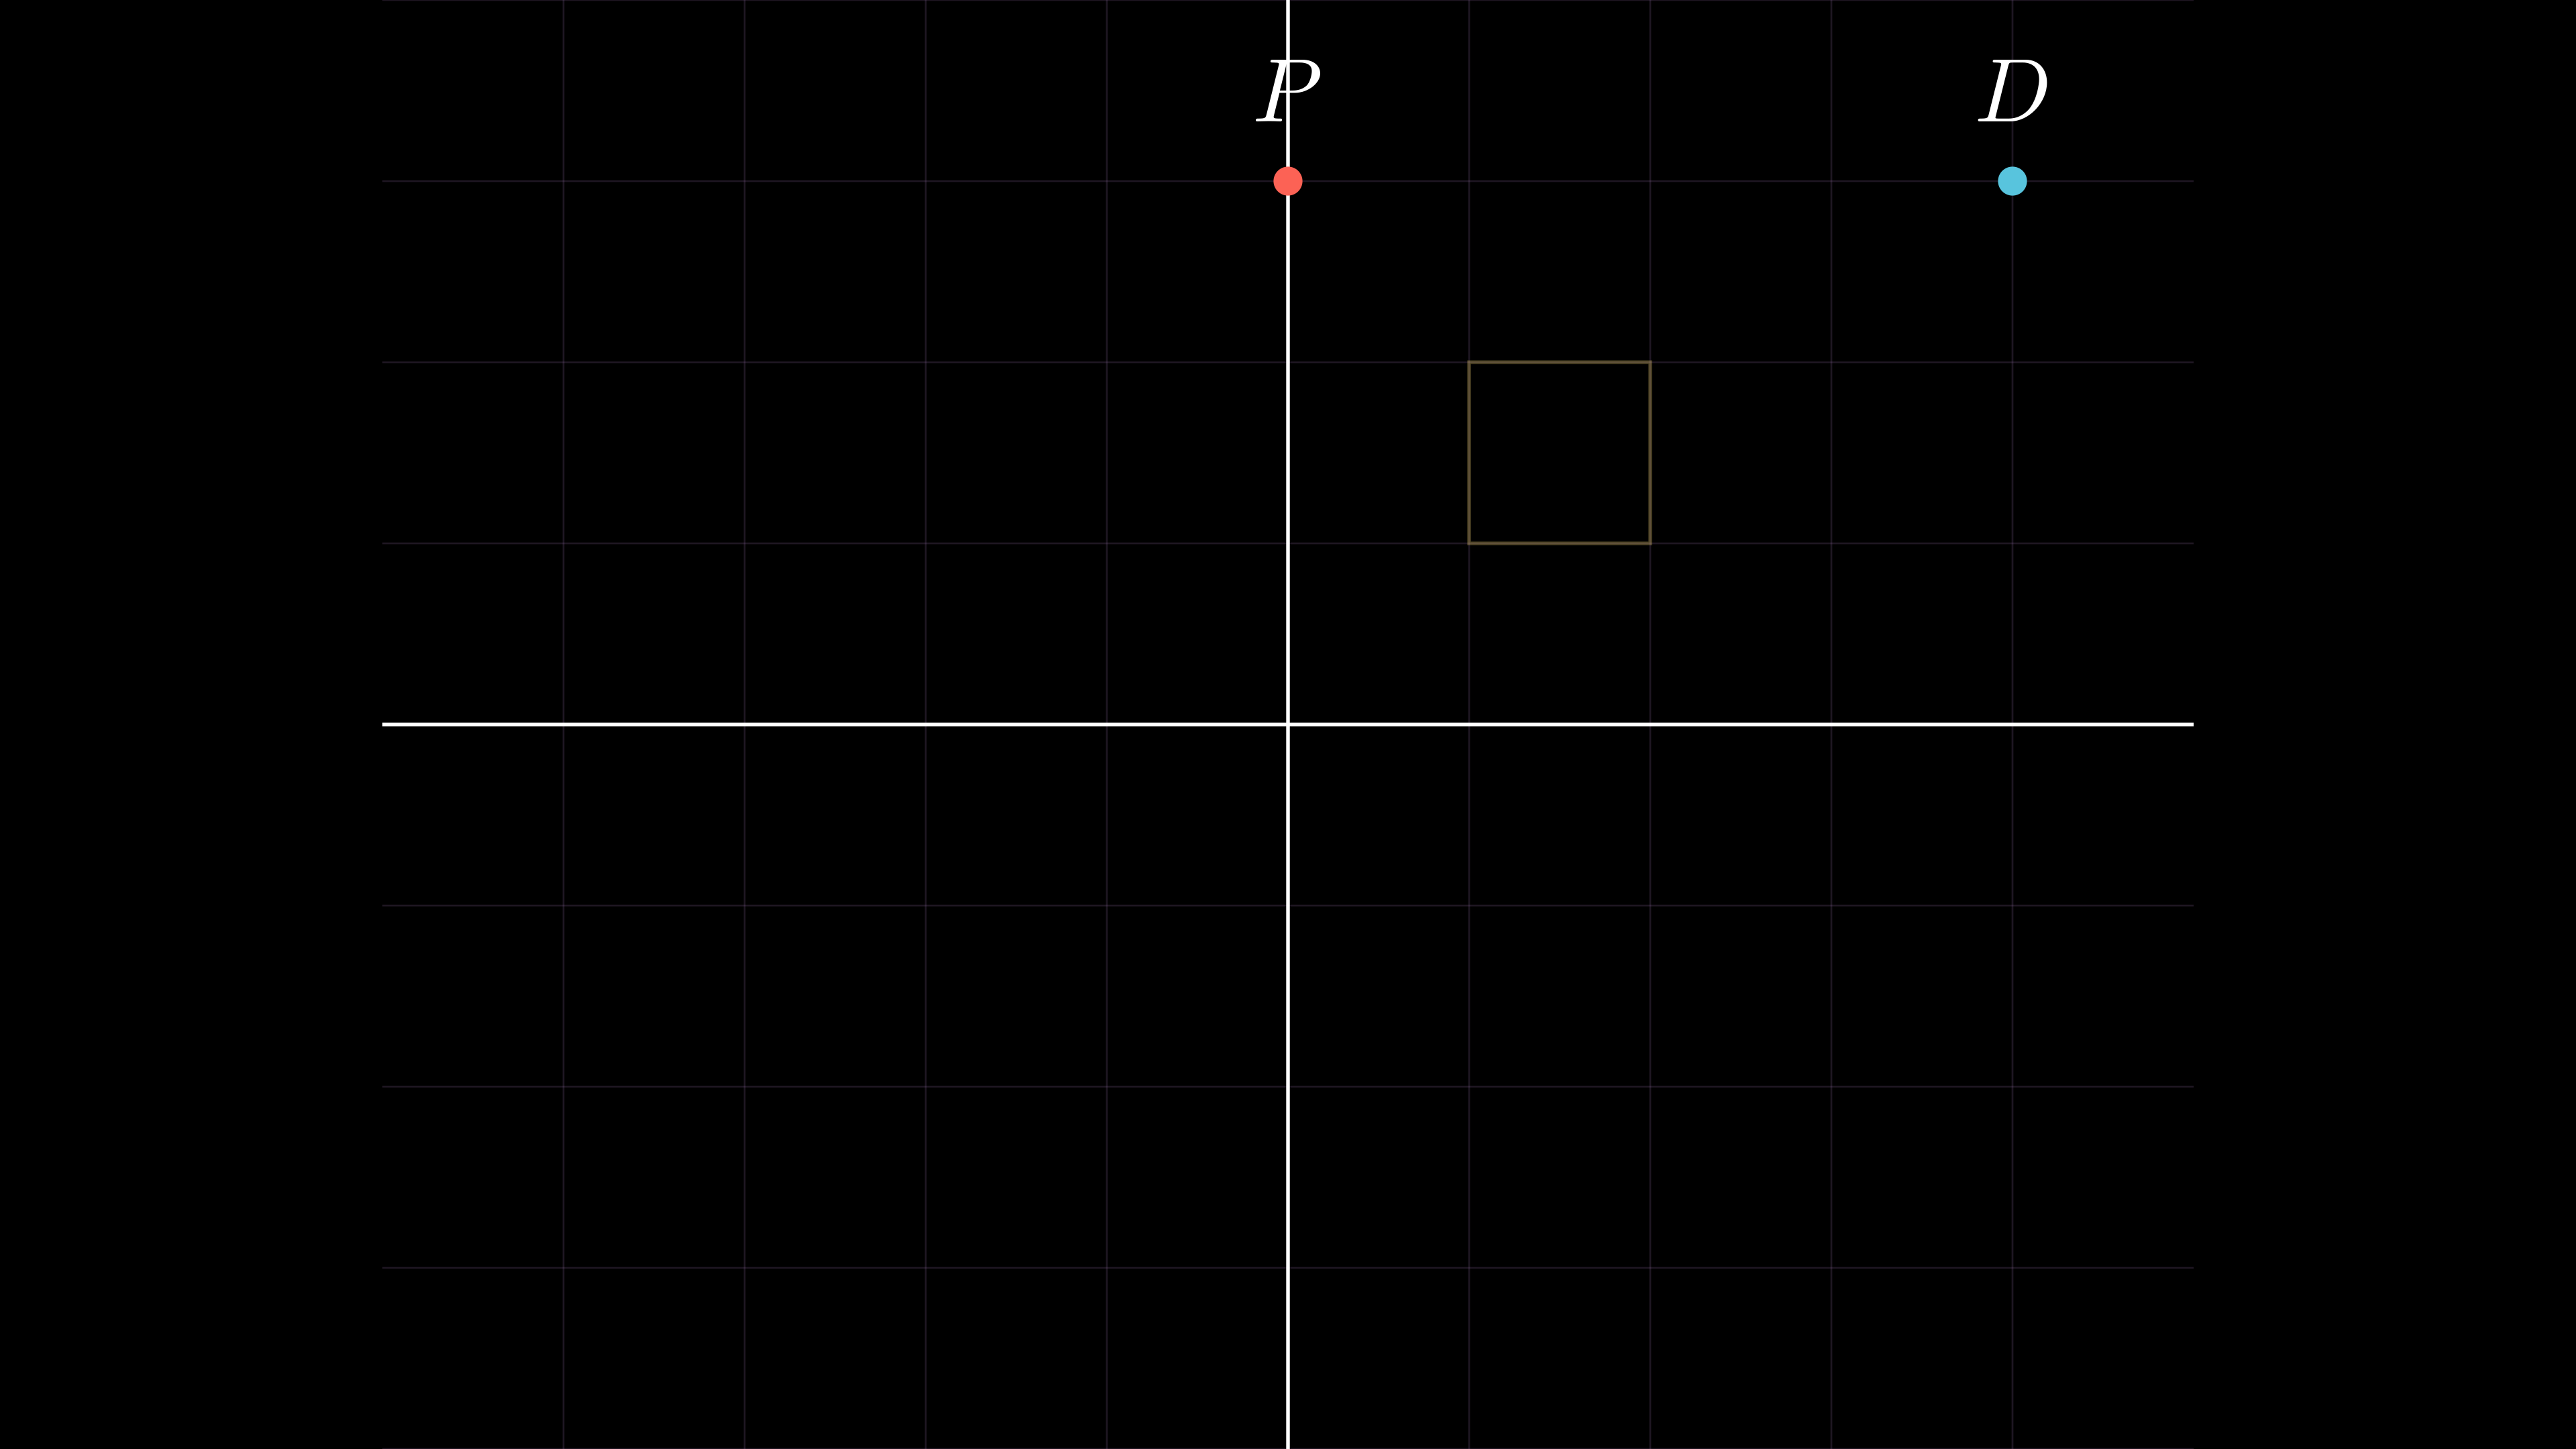
\includegraphics[width=\textwidth]{img/Phase1.png}
        \caption{Phase 1: Das reguläre, unverzerrte Grundraster.}
        \label{fig:phase1}
    \end{subfigure}
    \hfill
    \begin{subfigure}[t]{0.48\textwidth}
        \centering
        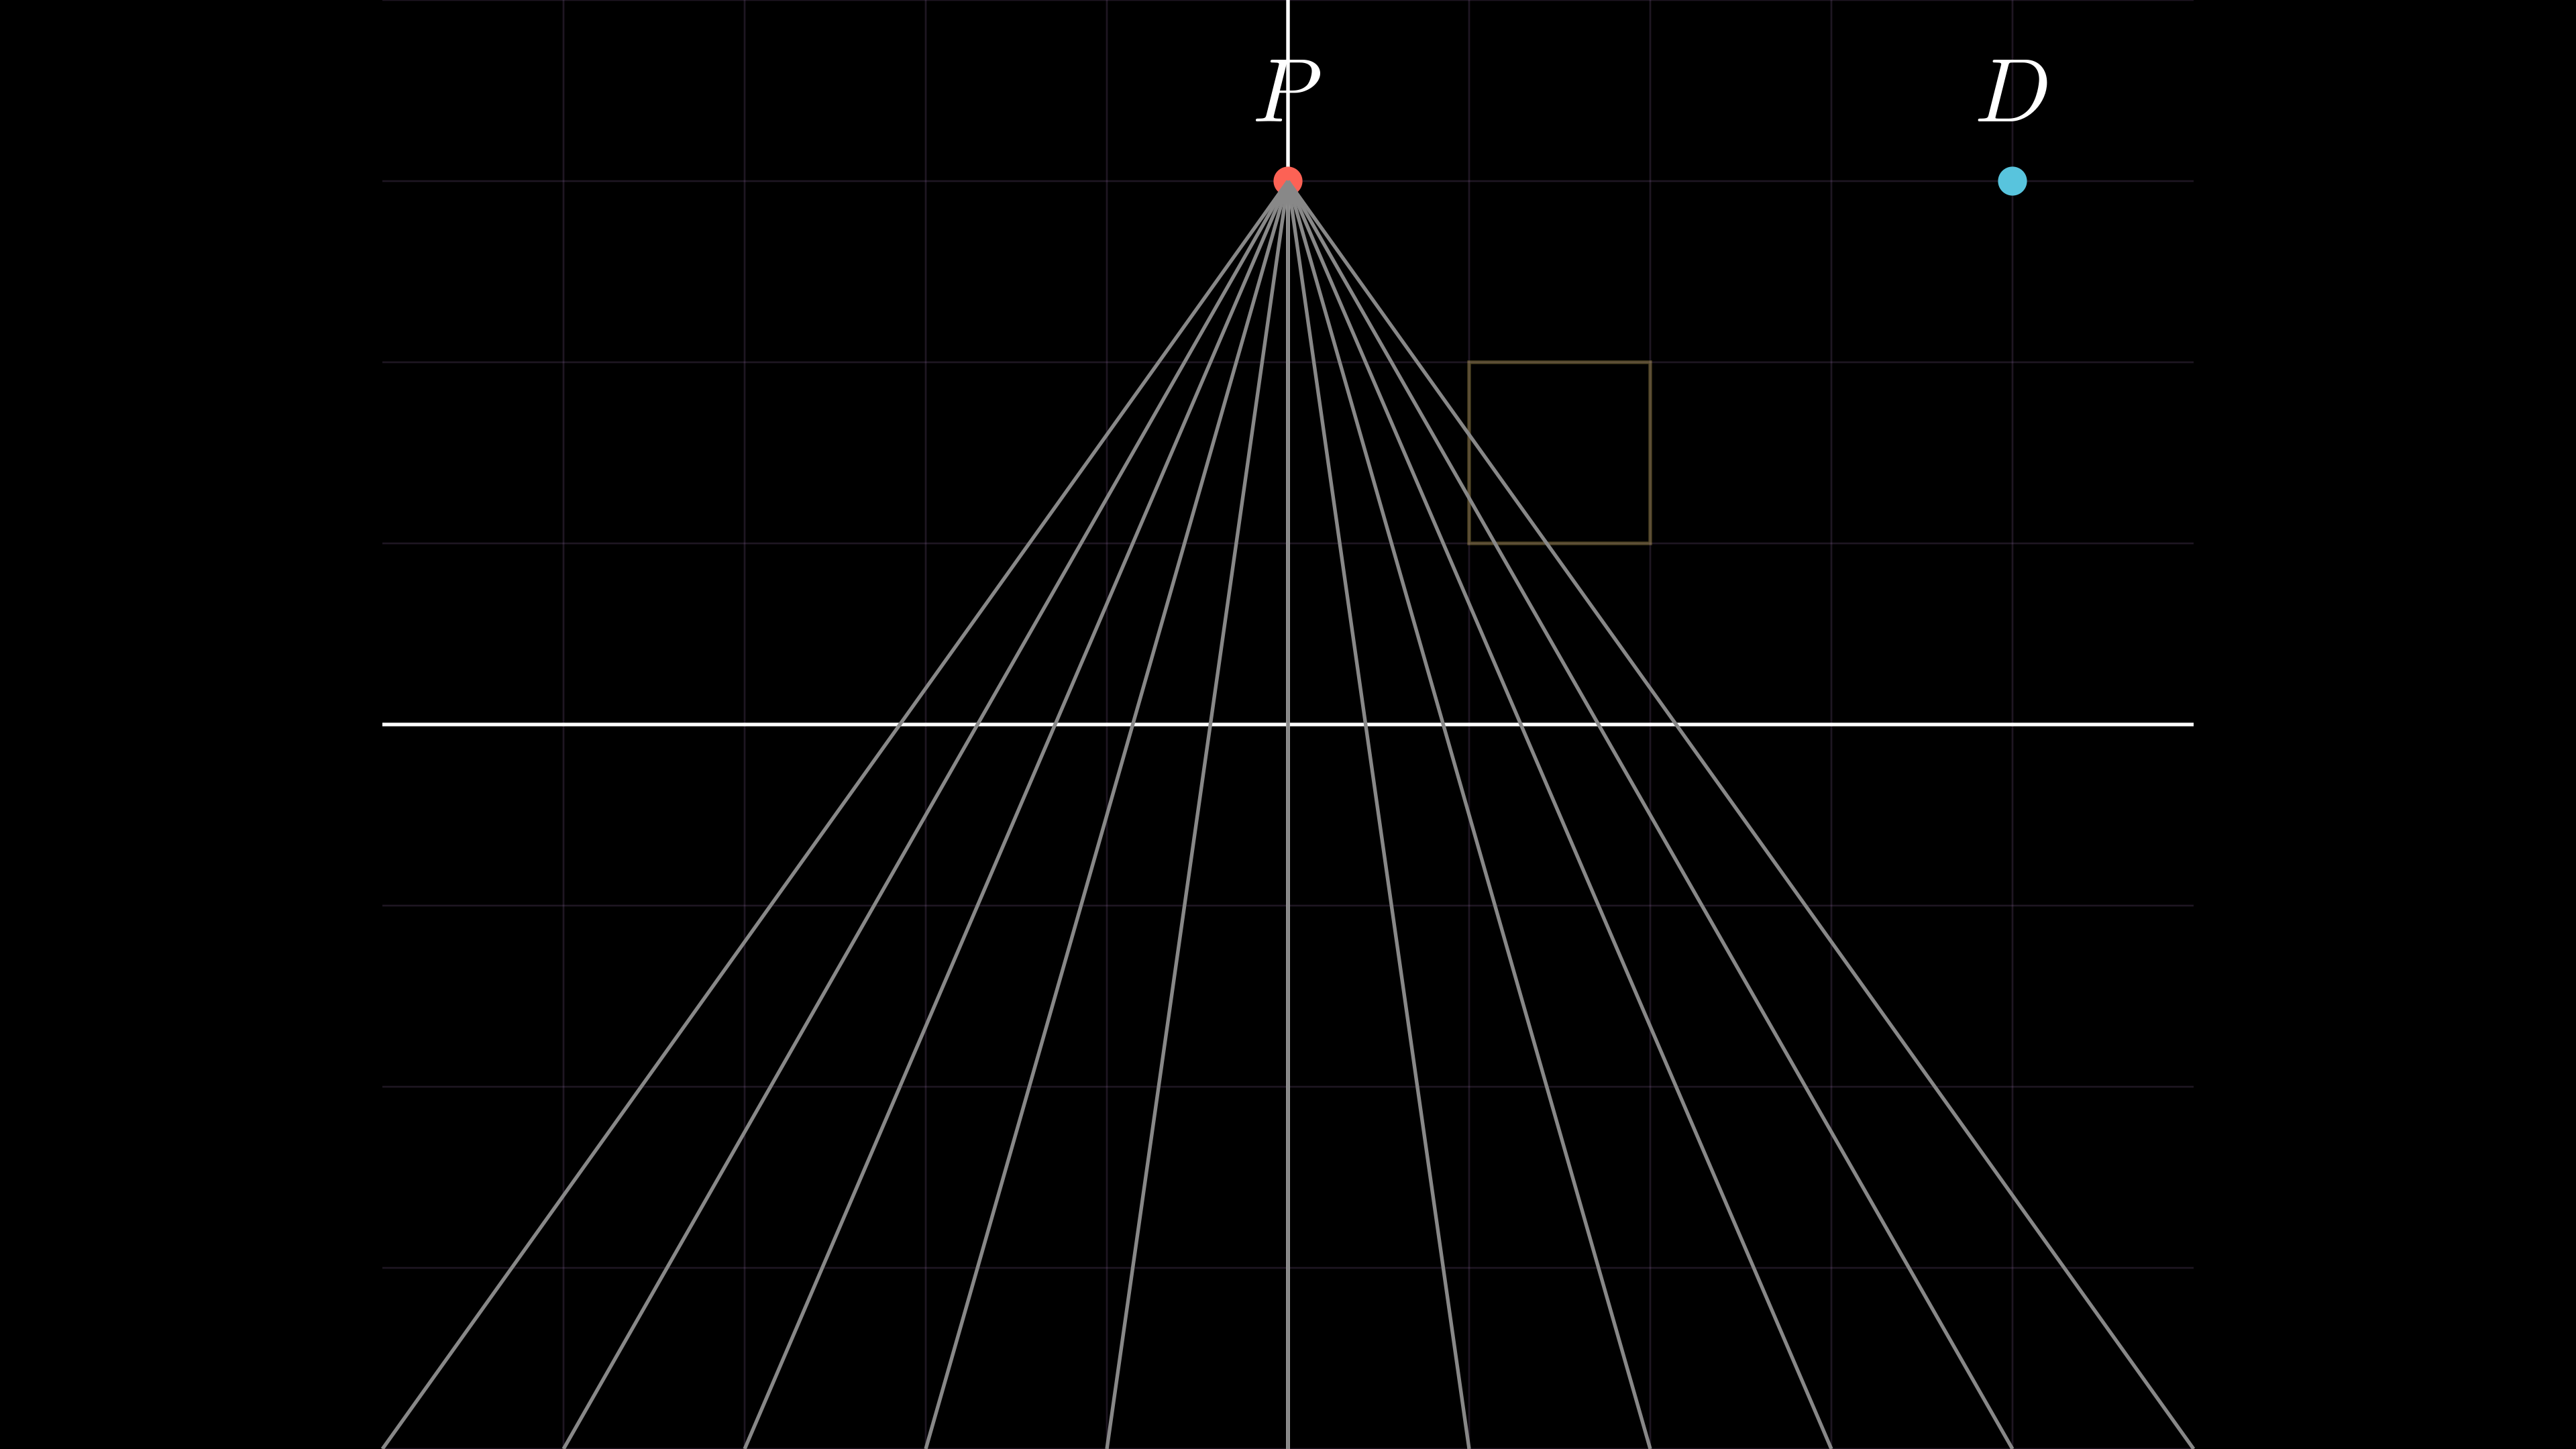
\includegraphics[width=\textwidth]{img/Phase2.png}
        \caption{Phase 2: Hauptfluchtpunkt und Distanzpunkt zur Tiefenbestimmung.}
        \label{fig:phase2}
    \end{subfigure}
    
    \vspace{0.5cm} % Abstand zwischen den Reihen
    
    % Zweite Reihe
    \begin{subfigure}[t]{0.48\textwidth}
        \centering
        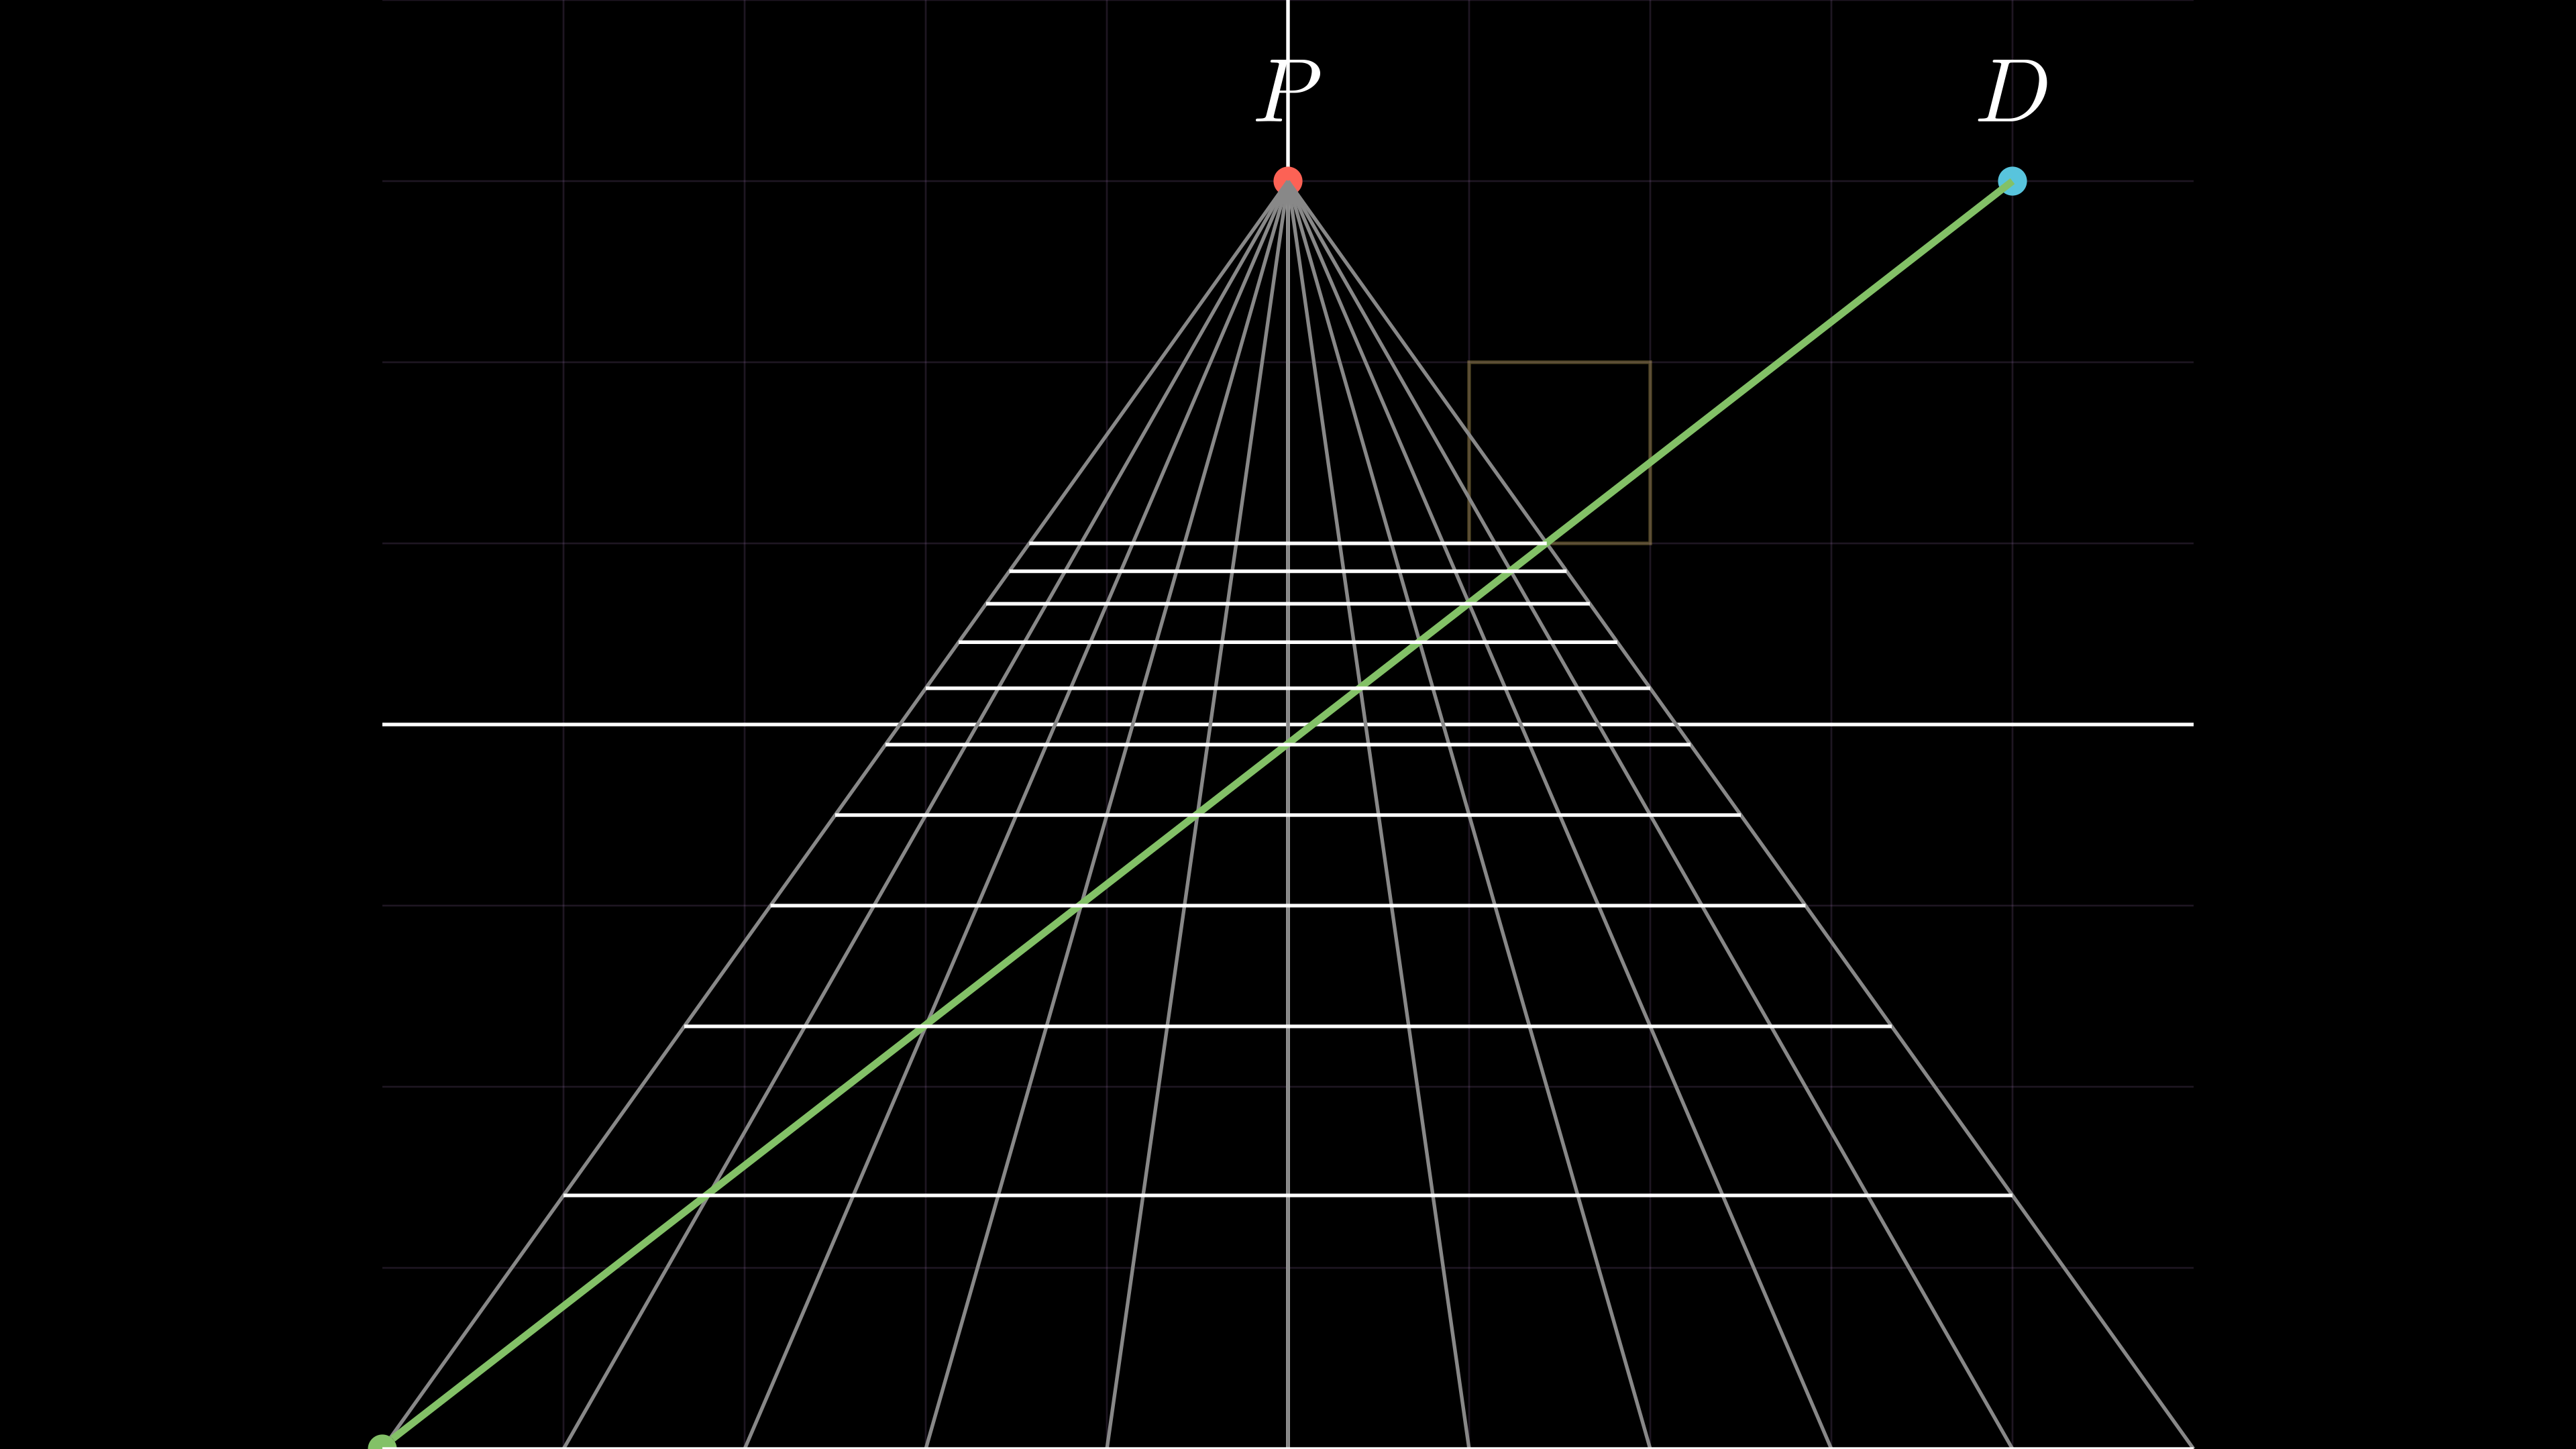
\includegraphics[width=\textwidth]{img/Phase3.png}
        \caption{Phase 3: Projektion der 45$^\circ$-Diagonalen für die Querlinien.}
        \label{fig:phase3}
    \end{subfigure}
    \hfill
    \begin{subfigure}[t]{0.48\textwidth}
        \centering
        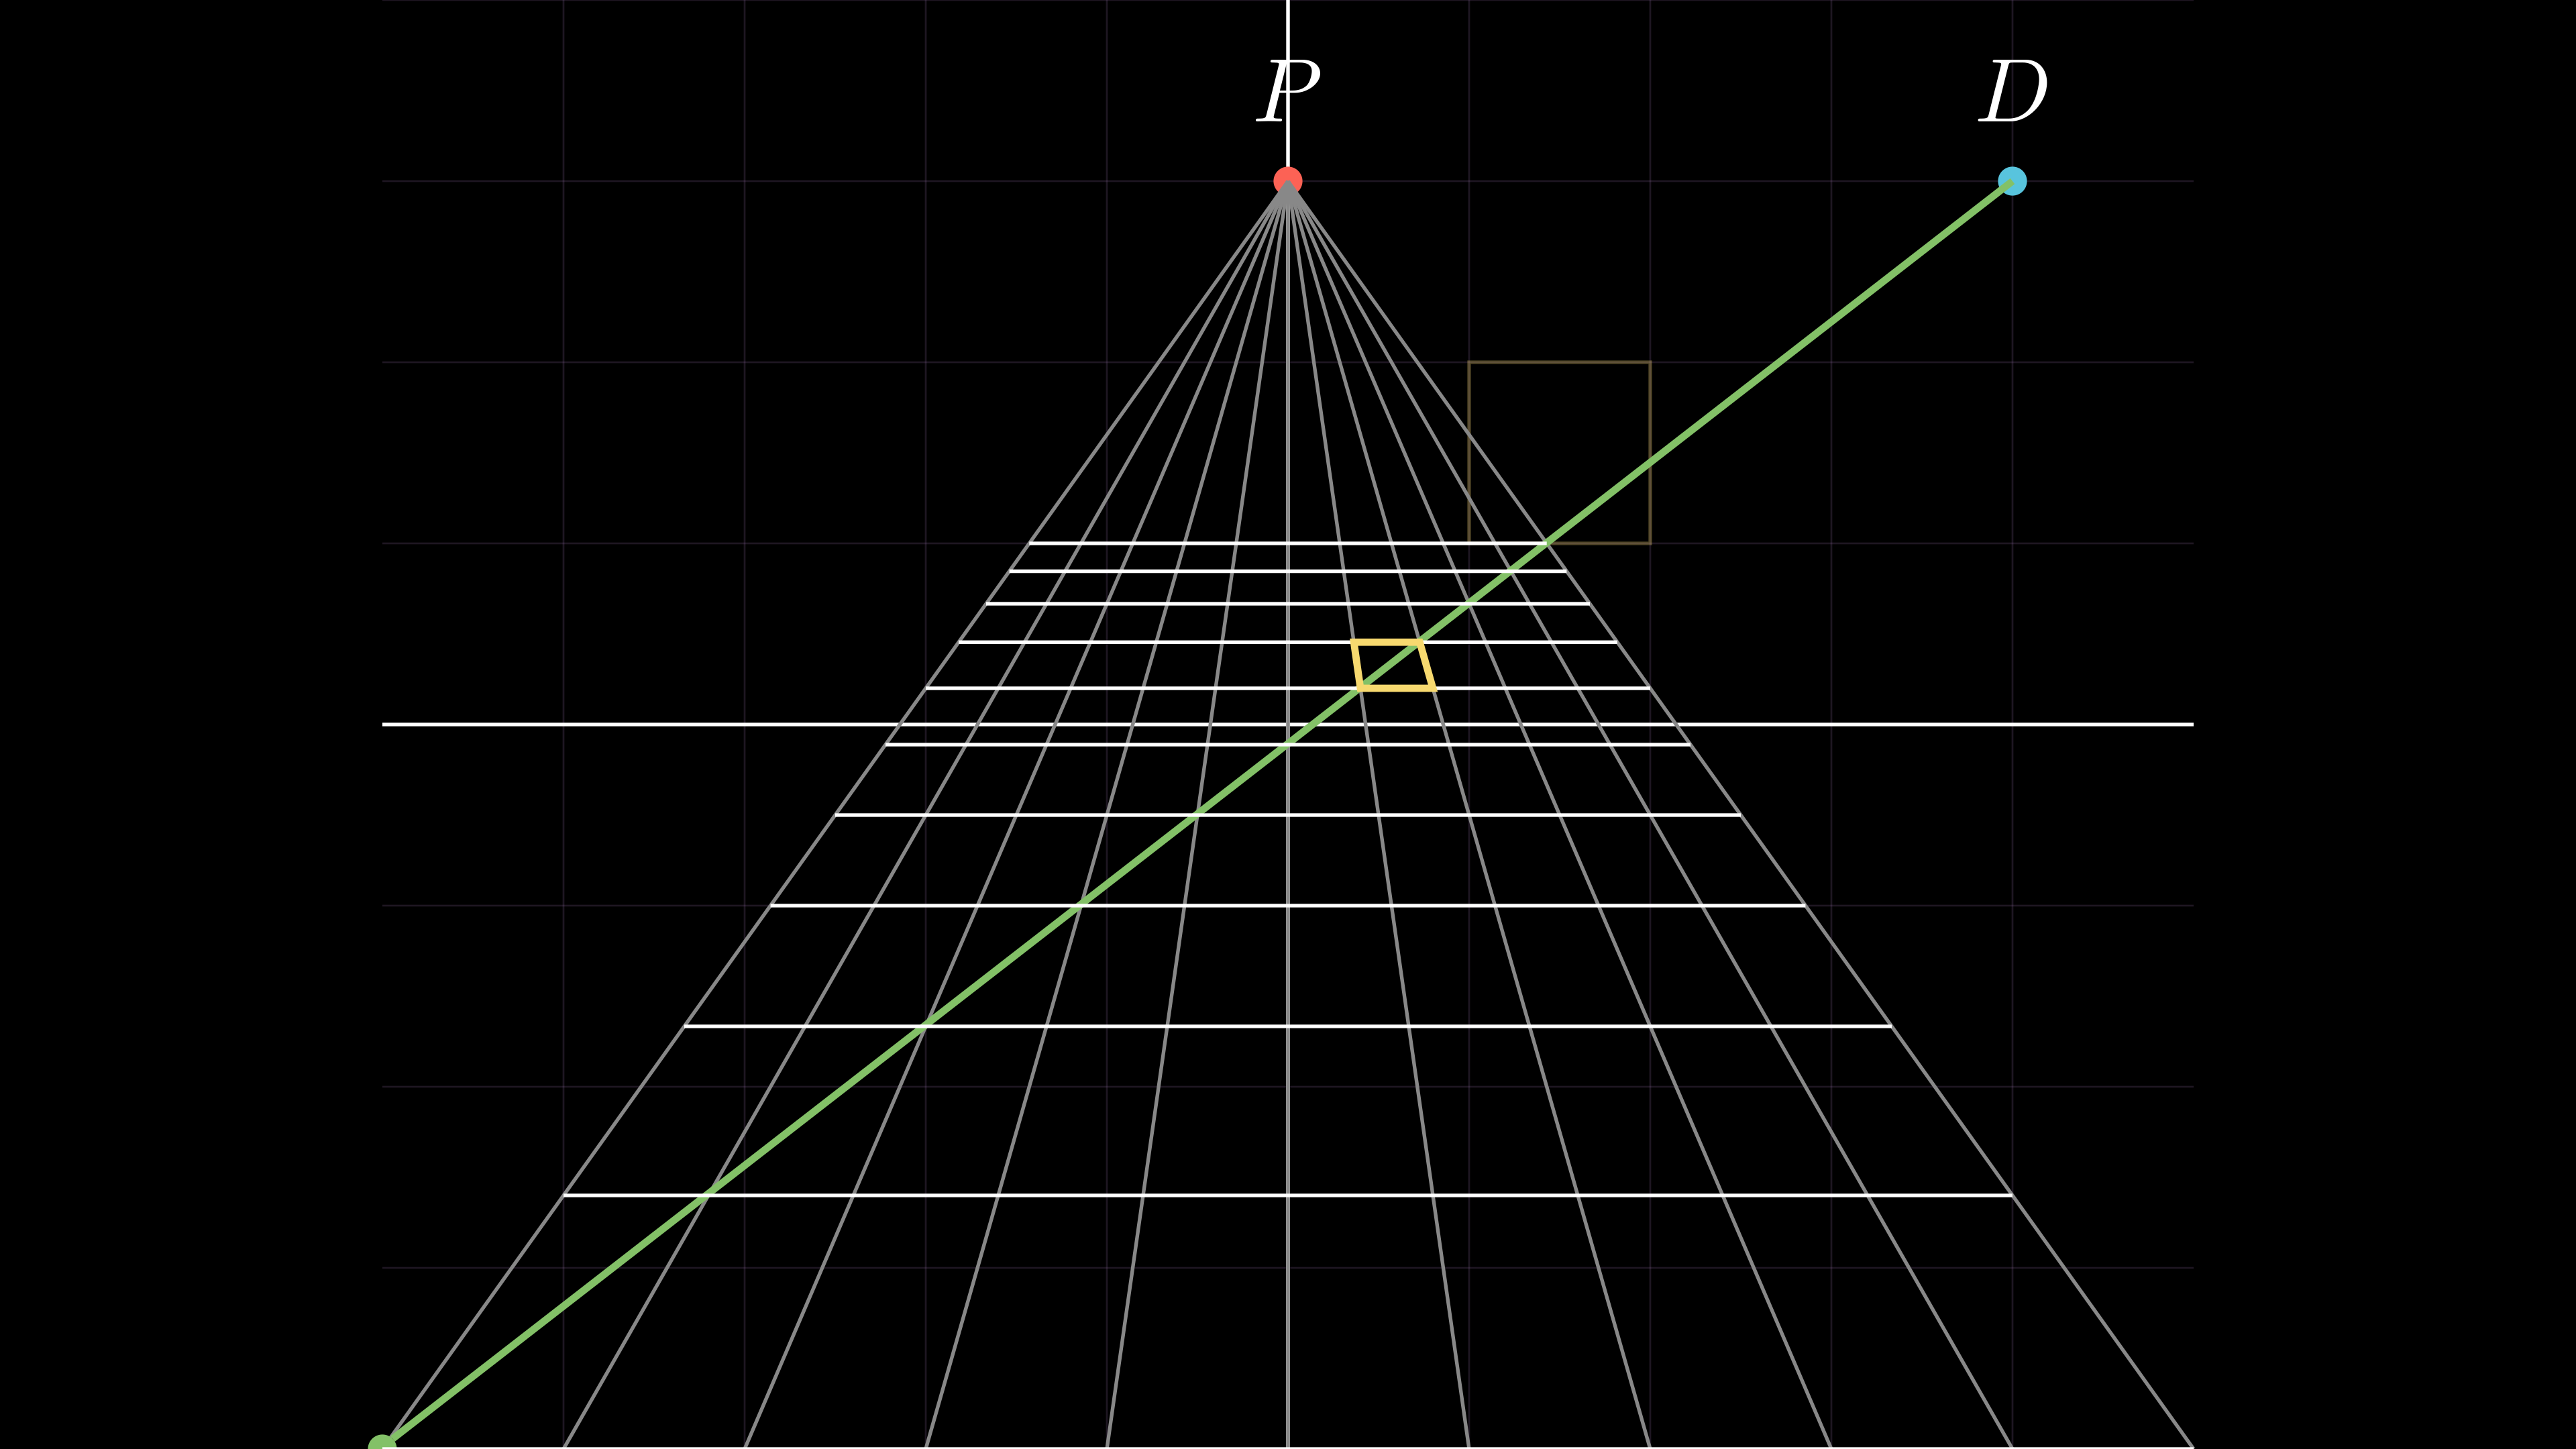
\includegraphics[width=\textwidth]{img/Phase4.png}
        \caption{Phase 4: Das finale, anamorphotisch verzerrte Netz.}
        \label{fig:phase4}
    \end{subfigure}
    
    \caption{Algorithmische Konstruktion der anamorphotischen Projektion nach Niceron mittels Manim.}
    \label{fig:manim_phasen}
\end{figure}

% Hier der Befehl zum direkten Einlesen der Datei
%\lstinputlisting[language=Python, caption={Manim Implementierung}, label={lst:manim_code}]{code/raster.py}

\newpage

\section{Fazit und Ausblick}

Die vorliegende Arbeit zeigt, dass die Entwicklung der Perspektive weit mehr war als die rein geometrische Anordnung von Objekten im Raum. Das Streben der Künstler und Mathematiker, Anatomie, Licht und Emotionen so lebensecht einzufangen - man denke hier nur an Vorzeigekünstler wie Leonardo Da Vinci -  als könne die Person jeden Moment aus dem Rahmen steigen, bildet heute die Grundlage für völlig neue Forschungszweige. So ermöglicht diese historische Detailtreue modernen Experten wie dem Pathologen Prof. Dr. Andreas Nerlich der Ludwig-Maximilians-Universität München die gezielte Analyse krankheitstypischer Merkmale auf alten Gemälden -- ein Verfahren, das bei flachen Darstellungen undenkbar wäre. Ein Beispiel ist Leonardo da Vincis \textit{Mona Lisa}, in welcher gelbliche Veränderungen am Augenlid (Xanthelasmen) und Lipome festzustellen sind, die auf eine Fettstoffwechselstörung hindeuten. \footnote{Vgl.: \cite{Morgenpost2026}} 

In diesem Sinne öffnete Leon Battista Alberti mit seiner historischen Analogie nicht nur ein Fenster, um die Realität als Momentaufnahme festzuhalten, sondern er spannte einen völlig neuen Raum der Möglichkeiten auf. Dieser Raum erstreckt sich bis in die Gegenwart: Er erlaubt es uns heute, die einst abstrakte Mathematik im Glanze moderner Werkzeuge wie Manim durch lebendige Animationen geradezu "`magisch"' neu zu vermitteln.

\newpage

\printbibheading[title={Quellenverzeichnis}] 

\printbibliography[keyword=haupt, heading=subbibliography, title={Hauptquellen}]
%\printbibliography[keyword=neben, heading=subbibliography, title={Nebenquellen}]
%\nocite{AdaPortrait, GeneralPlan}
%\printbibliography[keyword=bild, heading=subbibliography, title={Bildquellen}]



\end{document}